\scanpage{33}
\diagram{\[
\begin{array}{rll}
180\left\{\begin{array}{l}60=3\times20=2\times30\\120=4\times30=2\times60\end{array}\right.
&\begin{array}{l}f_{B,s}\\f_{\vec Q,a}\end{array}\\[1em]
420\left\{\begin{array}{l}
60=1\times60=\unsure{4|1}\times60\\
\inserted{120=1\times120=1\times120}\\
60=1\times60=5\times12\\
60=1\times60=3\times20\\
120=1\times120=6\times20
\end{array}\right.
&\begin{array}{l}\tau_{\pi,s}\\\inserted{\tau_r^0}\\\gamma_{\pi,s}\\\gamma''_{\pi,s}\\\gamma_r^0\end{array}\\[1em]
\begin{array}{r}1020\\\deleted{\unsure{900}}\end{array}
\left\{\begin{array}{l}
120=2\times60=1\times120\\
120=\unsure{2\times60}=2\times60\\
120=\unsure{1\times120}=2\times60\\
120=1\times120=2\times60\\
3\times120=\deleted{\unsure{2\times60=2\times60}}\inserted{3\times40=3\times40}\\
120=2\times60=2\times60\\
60=1\times60=2\times30
\end{array}\right.
&\left.\begin{array}{l}
\tau_{\pi,\rho}\\
\unsure{\gamma}_{\pi,\rho}\\
\unsure{\tau_r^1}\\
\gamma_r^1\\
\gamma_r^{1'}\\
\gamma_r^2\\
\gamma_r^{2'}
\end{array}\right\}\\[1em]
\begin{array}{r}\deleted{\unsure{1500}}\\\inserted{1620}\end{array}
=5\times60+\unsure{11}\times120
\end{array}
\]}
\[
\tau=\text{``twist''}\qquad
\gamma=\text{``gommage''}
\]

Programme de travail :

1) déterminer un syst. fondamental de relations entre les \(1620\) flèches du diagramme, \unsure{se partageant} \deleted{entre} \(14\) \deleted{\unsure{orbites}} sous \(\unsure{\mathfrak S}_K\) (aux \(542\) sommets, se partageant entre \(9\) orbites)

\margin{en particulier, écrire toutes les flèches comme composés de flèches ``provenant de la dimension relative \(\leq1\)''}

\deleted{\unsure{2) Réduire}}

2) Reprendre la question, en éliminant les sommets du niveau \(0\) (sauf \unsure{peut-on} ceux de type \(\unsure{\mathrm I_{20}|\mathrm{III}_2}\) ?),
\deleted{et \(\mathrm{II}_1\) (\unsure{qui se déduit par} \(\mathrm{II}_1\) (qui revient \unsure{à ceux} du type \(\mathrm{III}_1\).) --- mais Attention au twist \inserted{\(\mathrm{tw}_{1/6}\)} \unsure{relativement} : \(\mathrm{II}_1\) (\unsure{qui donne un Autom. du même type}))}

3) Eliminer de plus les pièces \deleted{\unsure{gauches}} ``tétraédrales'' \(\mathrm{II}_1\) --- et toutes les pièces qui ne semblent pas simplifier la présentation des relations.

\figure{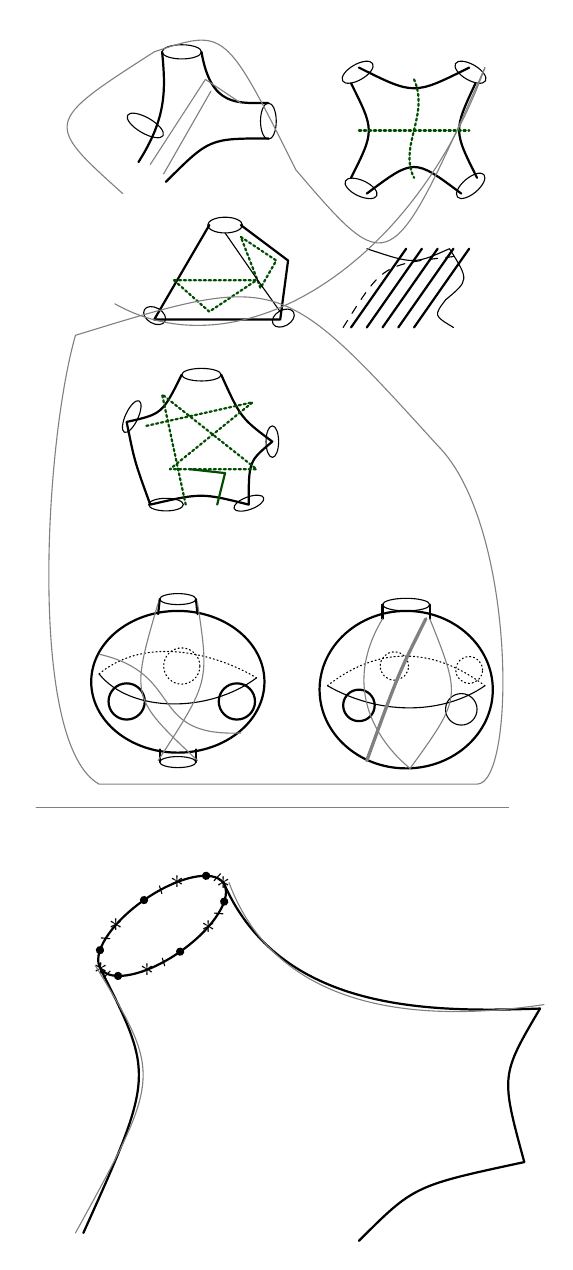
\begin{tikzpicture}[x=1cm,y=1cm,line cap=round,line join=round]
\begin{scope}[shift={(0,5)}]
\draw[thick] (-.5,1)..controls(-.45,.5)and(-.45,.15)..(-.8,-.4);
\draw[thick] (0,1)..controls(.12,.3)and(.45,.35)..(.85,.35);
\draw[thick] (.85,-.1)..controls(.1,-.1)..(-.45,-.65);
\draw (-.25,1) ellipse(.25 and .09);\draw[rotate=-30] (-.65,-.3) ellipse(.26 and .1);
\draw (.85,.12) ellipse(.1 and .23);
\draw[gray] (-.65,-.43)--(.05,.65)--(.5,.35);
\draw[gray] (-.48,-.55)--(.12,.5);
\end{scope}
\begin{scope}[shift={(2.7,5)}]
\draw[thick] (-.7,.8)..controls(0,.45)..(.7,.8);
\draw[thick] (.78,.6)..controls(.5,0)..(.8,-.6);
\draw[thick] (.6,-.8)..controls(0,-.35)..(-.6,-.8);
\draw[thick] (-.8,-.6)..controls(-.5,0)..(-.8,.6);
\draw[rotate=30](-.25,1)ellipse(.22 and .1);\draw[rotate=-30](.25,1)ellipse(.22 and .1);
\draw[rotate=-25](-.3,-.95)ellipse(.22 and .1);\draw[rotate=40](.1,-1)ellipse(.22 and .1);
\draw[green!30!black,densely dotted,thick] (-.7,0)--(.7,0);\draw[green!30!black,densely dotted,thick](0,.65)..controls(.2,.2)and(-.2,-.2)..(0,-.6);
\end{scope}
\begin{scope}[shift={(.3,3)}]
\draw[thick](-.2,.8)--(-.9,-.4)--(.7,-.4)--(.8,.35)--(.2,.8);
\draw (0,.8) ellipse(.22 and .1);\draw[rotate=-30](-.6,-.75)ellipse(.15 and .1);\draw[rotate=30](.45,-.7)ellipse(.15 and .1);
\draw[green!30!black,densely dotted,thick](-.65,.1)--(.4,.1)--(-.2,-.3)--(-.65,.1);
\draw[green!30!black,densely dotted,thick](.2,.65)--(.65,.35)--(.45,0)--(.2,.65);
\draw (0,.7)--(.45,.05)--(.7,-.3);
\end{scope}
\begin{scope}[shift={(2.5,3)}]
\draw[dashed](-.7,-.5)..controls(-.2,.3)..(.7,.4);
\draw(-.4,.5)..controls(.2,.3)..(.65,.5)..controls(.9,.1)..(.6,-.15)..controls(.45,-.35)..(.7,-.5);
\foreach \x in {-.6,-.4,-.2,0,.2}{\draw[thick](\x,-.5)--(\x+.7,.5);}
\end{scope}
\begin{scope}[shift={(0,.9)}]
\draw[thick](-.25,1)..controls(-.5,.5)..(-.95,.4)..controls(-.85,-.1)..(-.65,-.65)..controls(0,-.5)..(.6,-.65)..controls(.6,-.1)..(.9,.15)..controls(.5,.45)..(.25,1);
\draw(0,1)ellipse(.25 and .08);\draw[rotate=-25](-1,.05)ellipse(.08 and .22);\draw(.9,.15)ellipse(.08 and .2);
\draw(-.45,-.65)ellipse(.22 and .08);\draw[rotate=20](.35,-.8)ellipse(.2 and .08);
\draw[green!30!black,densely dotted,thick](-.7,.35)--(.65,.65)--(-.4,-.2)--(.7,-.2)--(-.5,.75)--(-.2,-.65);
\draw[green!30!black,thick](-.15,-.2)--(.3,-.25)--(.2,-.65);
\end{scope}
\begin{scope}[shift={(-.3,-2)}]
\draw[thick](0,0)ellipse(1.1 and .9);
\draw[thick](-.25,.86)--(-.23,1.05);\draw[thick](.25,.86)--(.23,1.05);\draw(0,1.05)ellipse(.23 and .07);
\draw[thick](-.23,-.86)--(-.23,-1.02);\draw[thick](.23,-.86)--(.23,-1.02);\draw(0,-1.02)ellipse(.23 and .07);
\draw[thick](-.65,-.25)circle(.23);\draw[thick](.75,-.25)circle(.23);\draw[densely dotted](.05,.2)circle(.23);
\draw(-1,.1)..controls(-.6,-.4)and(.4,-.4)..(1,.05);
\draw[densely dotted](-1,.1)..controls(-.4,.6)and(.5,.35)..(1,.05);
\draw[gray](-.25,1)..controls(-.6,-.2)..(.25,-1);\draw[gray](.25,1)..controls(.4,0)..(-.25,-1);
\draw[gray](-1,.35)..controls(.1,.1)and(-.4,-.7)..(.8,-.65);
\end{scope}
\begin{scope}[shift={(2.6,-2.1)}]
\draw[thick](0,0)ellipse(1.1 and 1);
\draw[thick](-.3,.9)--(-.3,1.08);\draw[thick](.3,.9)--(.3,1.08);\draw(0,1.08)ellipse(.3 and .08);
\draw[thick](-.6,-.2)circle(.2);\draw(.7,-.25)circle(.2);\draw[densely dotted](-.15,.3)circle(.18);\draw[densely dotted](.8,.25)circle(.17);
\draw(-1,.05)..controls(-.3,-.35)and(.5,-.3)..(1,.05);
\draw[densely dotted](-1,.05)..controls(-.3,.6)and(.4,.5)..(1,.05);
\draw[gray,very thick](.25,.9)..controls(-.1,.2)..(-.5,-.9);
\draw[gray](-.3,.9)..controls(-.9,-.1)and(-.2,-.8)..(.05,-1);
\draw[gray](.3,.9)..controls(.7,-.1)..(.05,-1);
\end{scope}
\draw[gray](-1.6,2.4)..controls(-2,1)and(-2.2,-2.8)..(-1.3,-3.3)--(3.5,-3.3)..controls(4,-3.3)and(4,0)..(3,1);
\draw[gray](-1.6,2.4)..controls(1,3.2)..(3,1);
\draw[gray](-1,4.2)..controls(-2,5.1)..(-.6,6)..controls(.3,6.3)..(1.2,4.5)..controls(2.4,3.1)..(3.6,5.8);
\draw[gray](-1.1,2.8)..controls(.5,1.9)and(2.7,3.3)..(3.6,5.8);
\draw[gray](-2.1,-3.6)--(3.9,-3.6);
\begin{scope}[shift={(-.5,-5.1)},rotate=35]
\draw[thick](0,0)ellipse(.95 and .4);
\foreach \a in {0,60,120,180,240,300}{\node at ({.95*cos(\a)},{.4*sin(\a)}) {$*$};}
\foreach \a in {30,90,150,210,270,330}{\fill ({.95*cos(\a)},{.4*sin(\a)})circle(1.5pt);}
\foreach \a in {15,75,135,195,255,315}{\draw ({.9*cos(\a)},{.35*sin(\a)})--({1.02*cos(\a)},{.45*sin(\a)});}
\end{scope}
\draw[thick](-1.28,-5.65)..controls(-.6,-7)..(-1.5,-9);
\draw[thick](.28,-4.55)..controls(1,-6.2)and(2.9,-6.2)..(4.3,-6.15);
\draw[thick](4.3,-6.15)..controls(3.8,-7)..(4.1,-8.1);
\draw[thick](4.1,-8.1)..controls(2.7,-8.4)..(2,-9.1);
\draw[gray](-1.35,-5.6)..controls(-.5,-7)..(-1.6,-9);
\draw[gray](.35,-4.55)..controls(1,-6.3)and(3,-6.3)..(4.35,-6.1);
\end{tikzpicture}}

\unsure{\texttt{//}}\illegible{6}

\unsure{\texttt{//}}\illegible{4}\unsure{\texttt{DISP=}}\illegible{2}

\unsure{\texttt{//}}\illegible{3}\unsure{\texttt{SYSPRINT}}\illegible{2}

\unsure{\texttt{//}}\illegible{3}\unsure{\texttt{VOL=SER}}\illegible{2}

\unsure{\texttt{//PL1}}\ \unsure{\texttt{DD DSN=}}\illegible{4}

\unsure{\texttt{//}}\illegible{5}

\unsure{\texttt{//}}\illegible{5}

\unsure{\texttt{//}}\illegible{4}\unsure{\texttt{DISP=(OLD,DELETE)}}

\unsure{\texttt{//}}\illegible{3}\unsure{\texttt{SPACE=(CYL,}}\illegible{2}

\unsure{\texttt{//}}\illegible{4}

\unsure{\texttt{//}}\illegible{4}

\unsure{\texttt{//}}\illegible{3}\unsure{\texttt{DELETE}}

\unsure{\texttt{//}}\illegible{4}\unsure{\texttt{VOL=SER}}\illegible{2}

\unsure{\texttt{//}}\illegible{3}\unsure{\texttt{SPACE=(CYL,}}\illegible{2}

\unsure{\texttt{//}}\illegible{3}\unsure{\texttt{DCB=}}\illegible{2}

\unsure{\texttt{//}}\illegible{3}\unsure{\texttt{DISP=(OLD,DELETE)}}

\unsure{\texttt{//}}\illegible{3}

\unsure{\texttt{//}}\illegible{4}

\unsure{\texttt{//}}\illegible{3}\unsure{\texttt{DCB=(RECFM=VBS,LRECL=20000,BLKSIZE=6440)}}

\unsure{\texttt{//}}\illegible{2}\unsure{\texttt{DISP=(CATLG),SPACE=(TRK,}}\illegible{2}

\unsure{\texttt{//}}\illegible{2}\unsure{\texttt{UNIT=SYSDA,VOL=SER=}}\illegible{1}

\unsure{\texttt{//}}\illegible{3}\unsure{\texttt{DCB=}}\illegible{2}

\unsure{\texttt{//}}\illegible{3}\unsure{\texttt{DISP=(MOD,DELETE)}}

\unsure{\texttt{//}}\illegible{2}\unsure{\texttt{DCB=(RECFM=VBS,LRECL=20000,BLKSIZE=6440)}}

\unsure{\texttt{//}}\illegible{2}\unsure{\texttt{UNIT=SYSDA,VOL=SER=}}\illegible{1}

\unsure{\texttt{//}}\illegible{2}\unsure{\texttt{DISP=(OLD,DELETE)}}

\unsure{\texttt{//}}\illegible{2}\unsure{\texttt{DSN=CHJ2.}}\illegible{1}

\unsure{\texttt{//}}\illegible{2}\unsure{\texttt{DISP=(OLD,DELETE)}}

\mspage{32}
